\section{Cyclic Buffer Dependency is Insufficient for Deadlock}\label{sec:casestudy}

\subsection{Single Flow in a Loop}

A routing loop leads to cyclic buffer dependency if a flow is trapped in the loop.
Such cyclic buffer dependency may not be sufficient for forming a deadlock. The flow
sending rate, draining rate and the TTL (time-to-live) of packets determine whether
there will be deadlock and how fast the deadlock forms.


\subsection{Multiple flows}



In this part, we present our simulation study about three deadlock cases, and demonstrate that 1) cyclic buffer dependency is not a sufficient and necessary condition for deadlock; 2) simultaneous cyclic pause is not sufficient to create a permanent deadlock.

\begin{figure*}[t]
%\vspace{-0.1in}
\centering

\subfloat[short for lof][Topology and flows.] {
    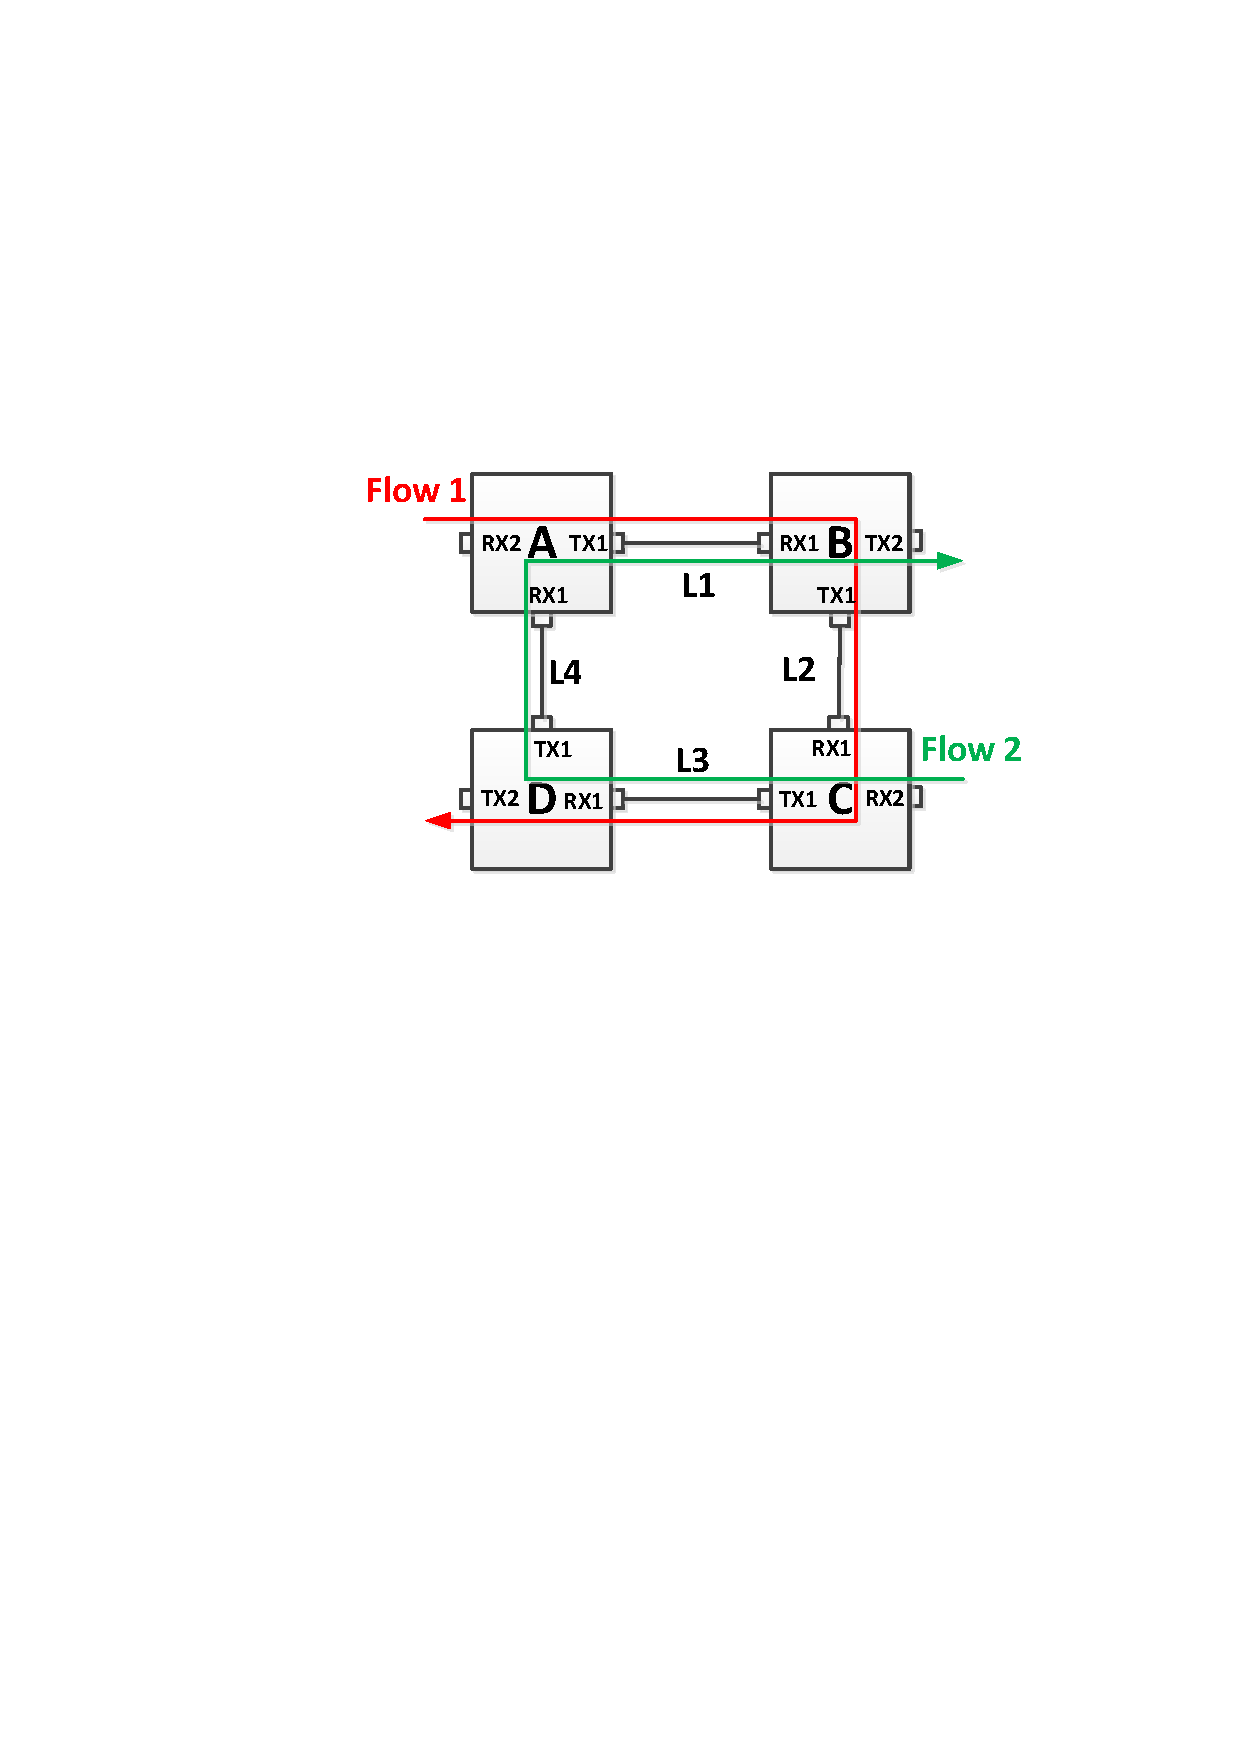
\includegraphics[width=0.4\textwidth] {figs/case1_topo.pdf}
}
\subfloat[short for lof][Buffer dependency graph.]{
    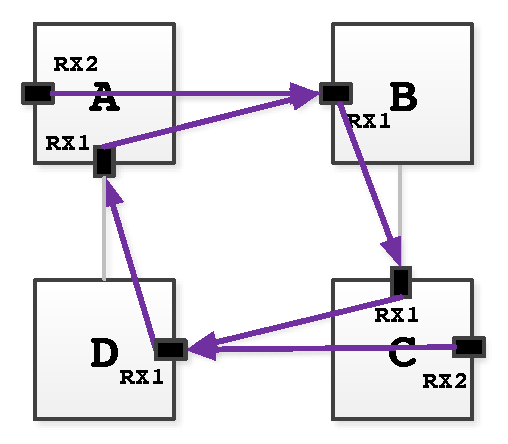
\includegraphics[width=0.24\textwidth] {figs/case1_buffer_dependency.pdf}
}
\subfloat[short for lof][Pause events at four links.]{
    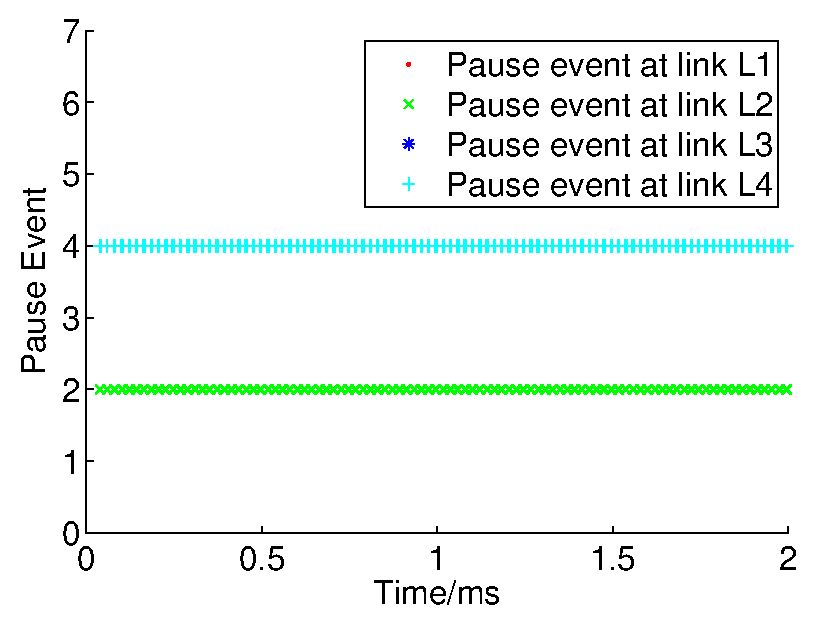
\includegraphics[width=0.3\textwidth] {figs/case1_pause.eps}
}

\subfloat[short for lof][Buffer occupancy at switch A.] {
    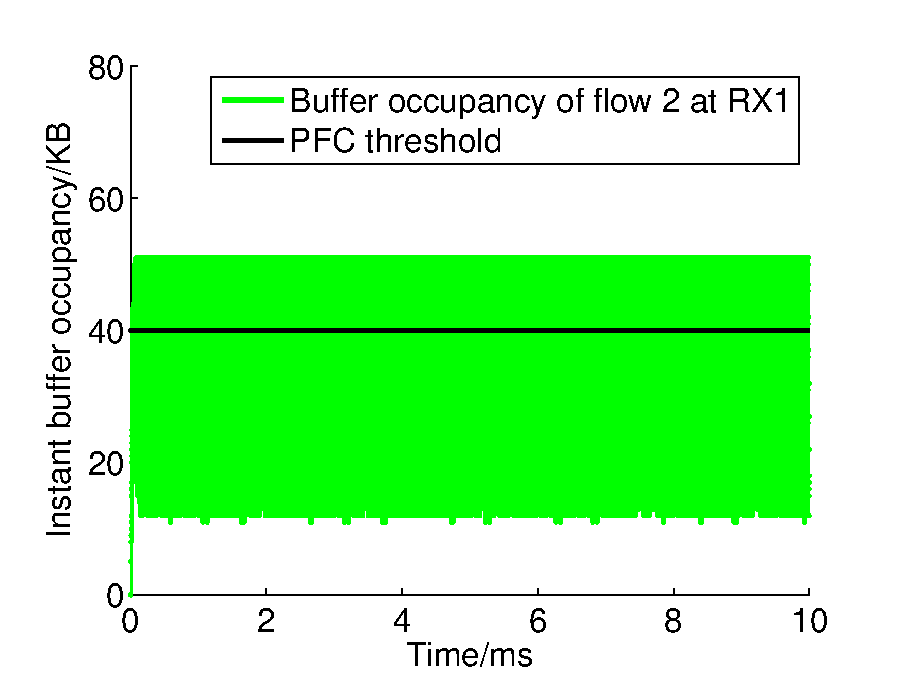
\includegraphics[width=0.25\textwidth] {figs/case1_buffer_occupancy_A.eps}
}
\subfloat[short for lof][Buffer occupancy at switch B.] {
    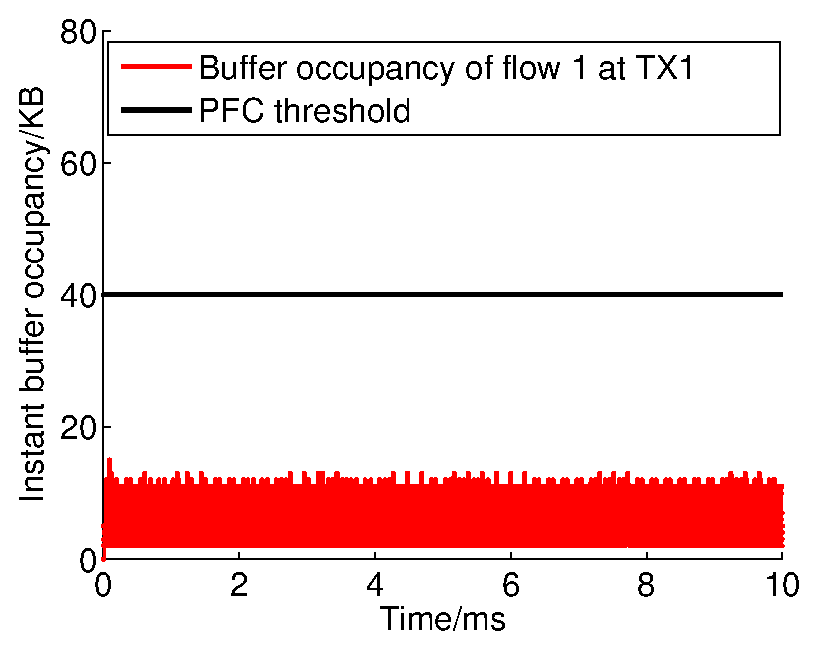
\includegraphics[width=0.25\textwidth] {figs/case1_buffer_occupancy_B.eps}
}
\subfloat[short for lof][Buffer occupancy at switch C.] {
    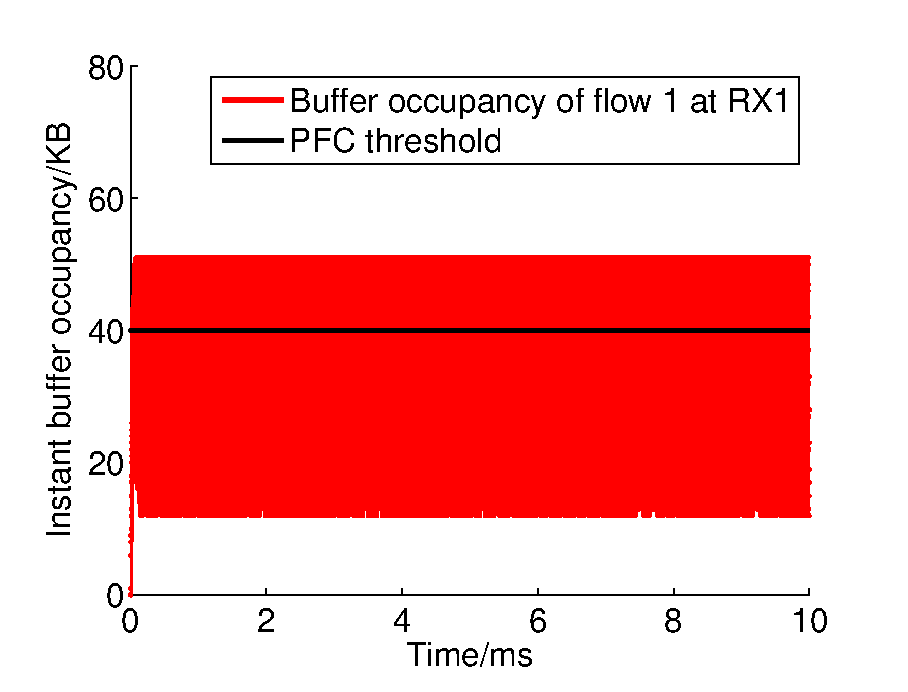
\includegraphics[width=0.25\textwidth] {figs/case1_buffer_occupancy_C.eps}
}
\subfloat[short for lof][Buffer occupancy at switch D.] {
    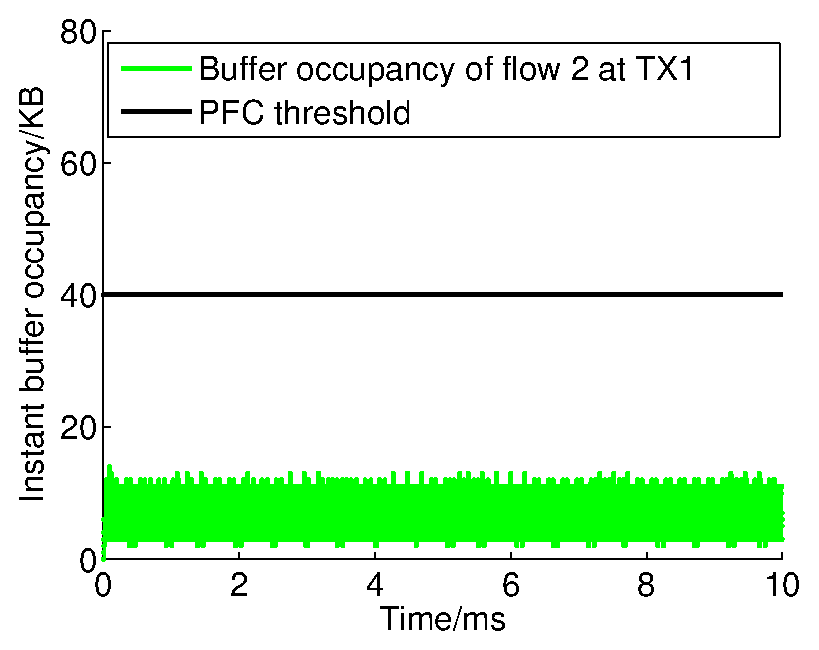
\includegraphics[width=0.25\textwidth] {figs/case1_buffer_occupancy_D.eps}
}

\caption{Deadlock case 1.}\label{fig:case1}

\end{figure*}

 \textbf{Simulation setup}: To create a well controlled experimental environment for deadlock analysis, we did our deadlock case study using packet-level NS-3 simulations. 
 
 In our modified NS-3 simulator, we implement PFC protocol (i.e., IEEE 802.1 Qbb protocol). Note that most modern commodity switches are output-queued, while PFC works in a per ingress queue fashion. Basically, for each ingress queue, the switch will maintain a counter to track its instant virtual queue length (i.e., bytes of buffered packets received by this ingress queue). Once the queue length of an ingress queue exceeds the pre-configured PFC threshold, a pause frame will be sent to the corresponding upstream device. The upstream device then stop sending any packet to this ingress queue unless 1) the pause frame has expired; 2) or it has received a resume frame from this ingress queue.
 
 In our simulations, link capacity of all links is 40Gbps. All the switches have 12MB buffer. PFC threshold is statically set to 40KB for each ingress queue.


\begin{figure*}[t]
%\vspace{-0.1in}
\centering

\subfloat[short for lof][Topology and flows.] {
    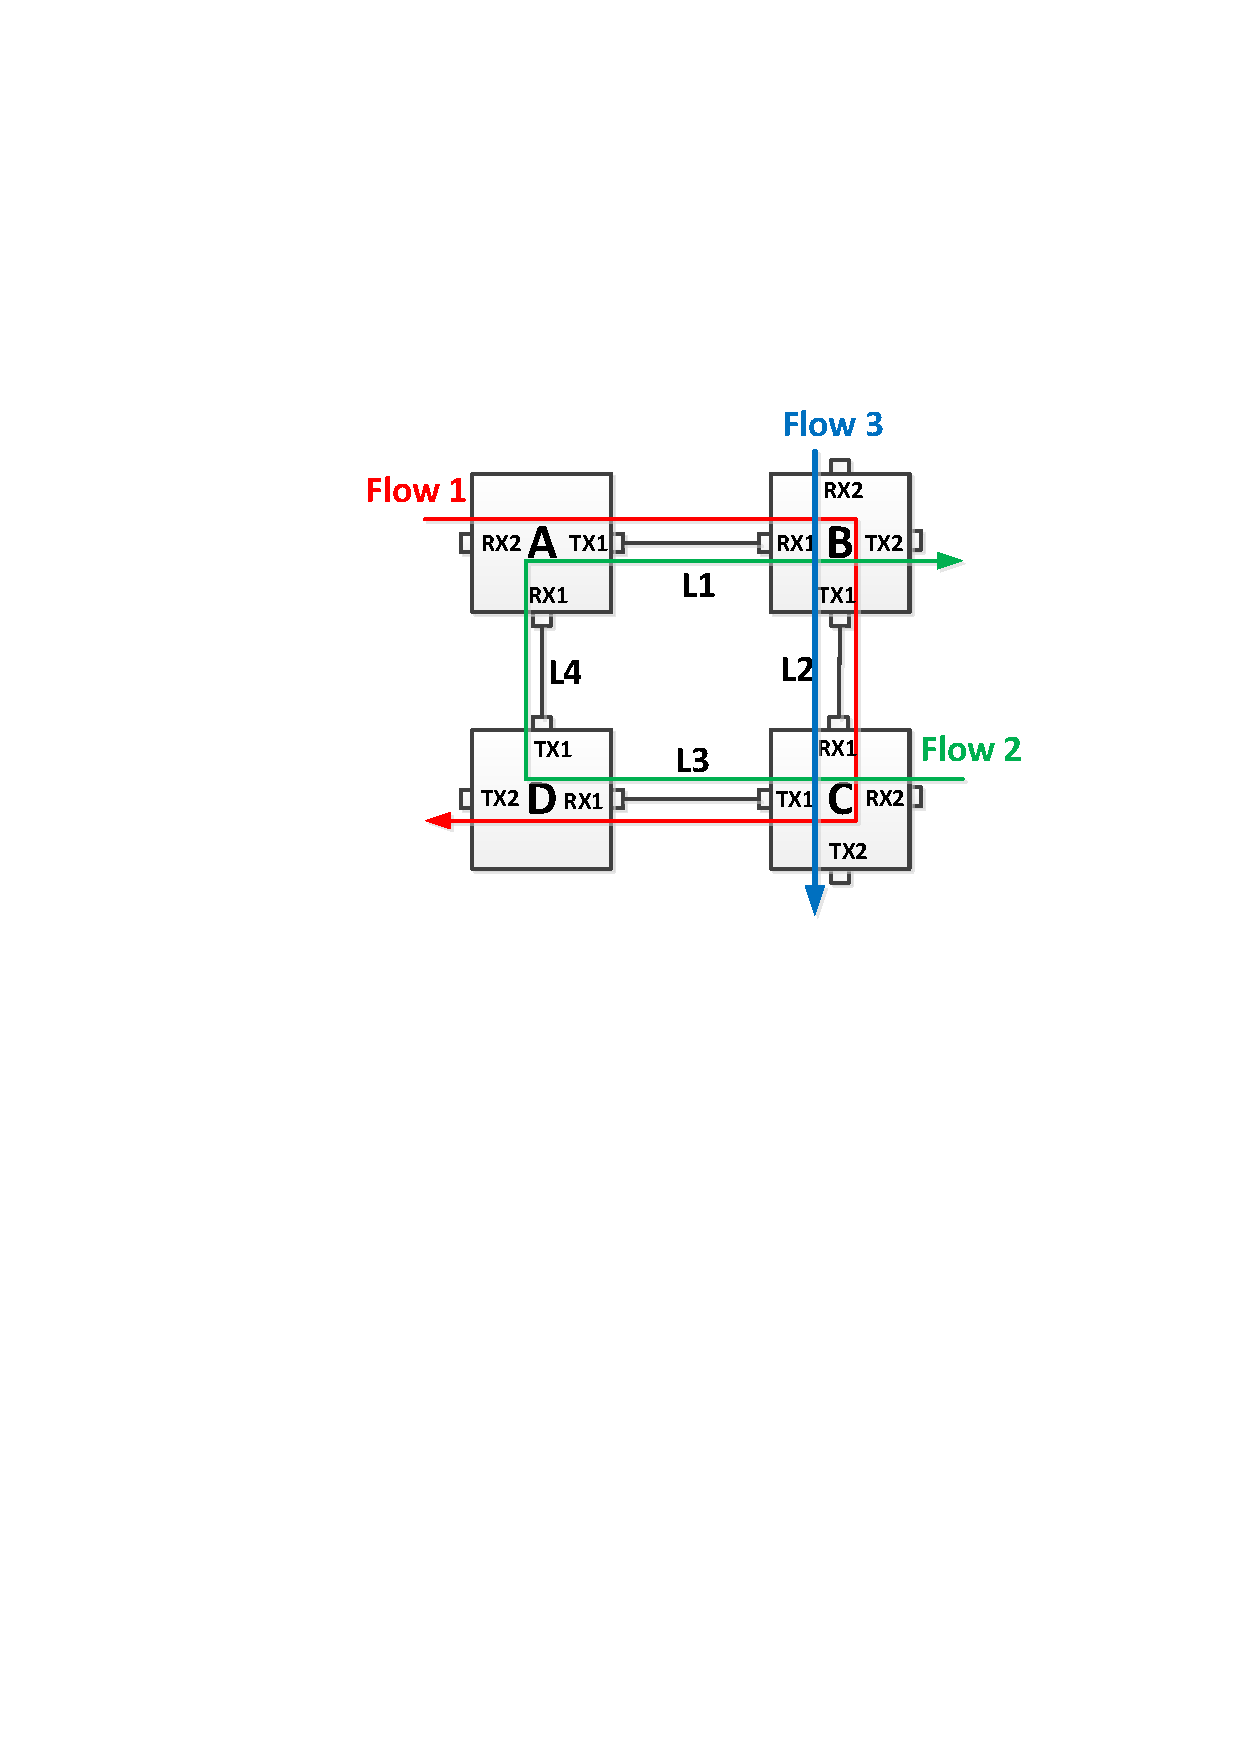
\includegraphics[width=0.37\textwidth] {figs/case2_topo}
}
\subfloat[short for lof][Buffer dependency graph.]{
    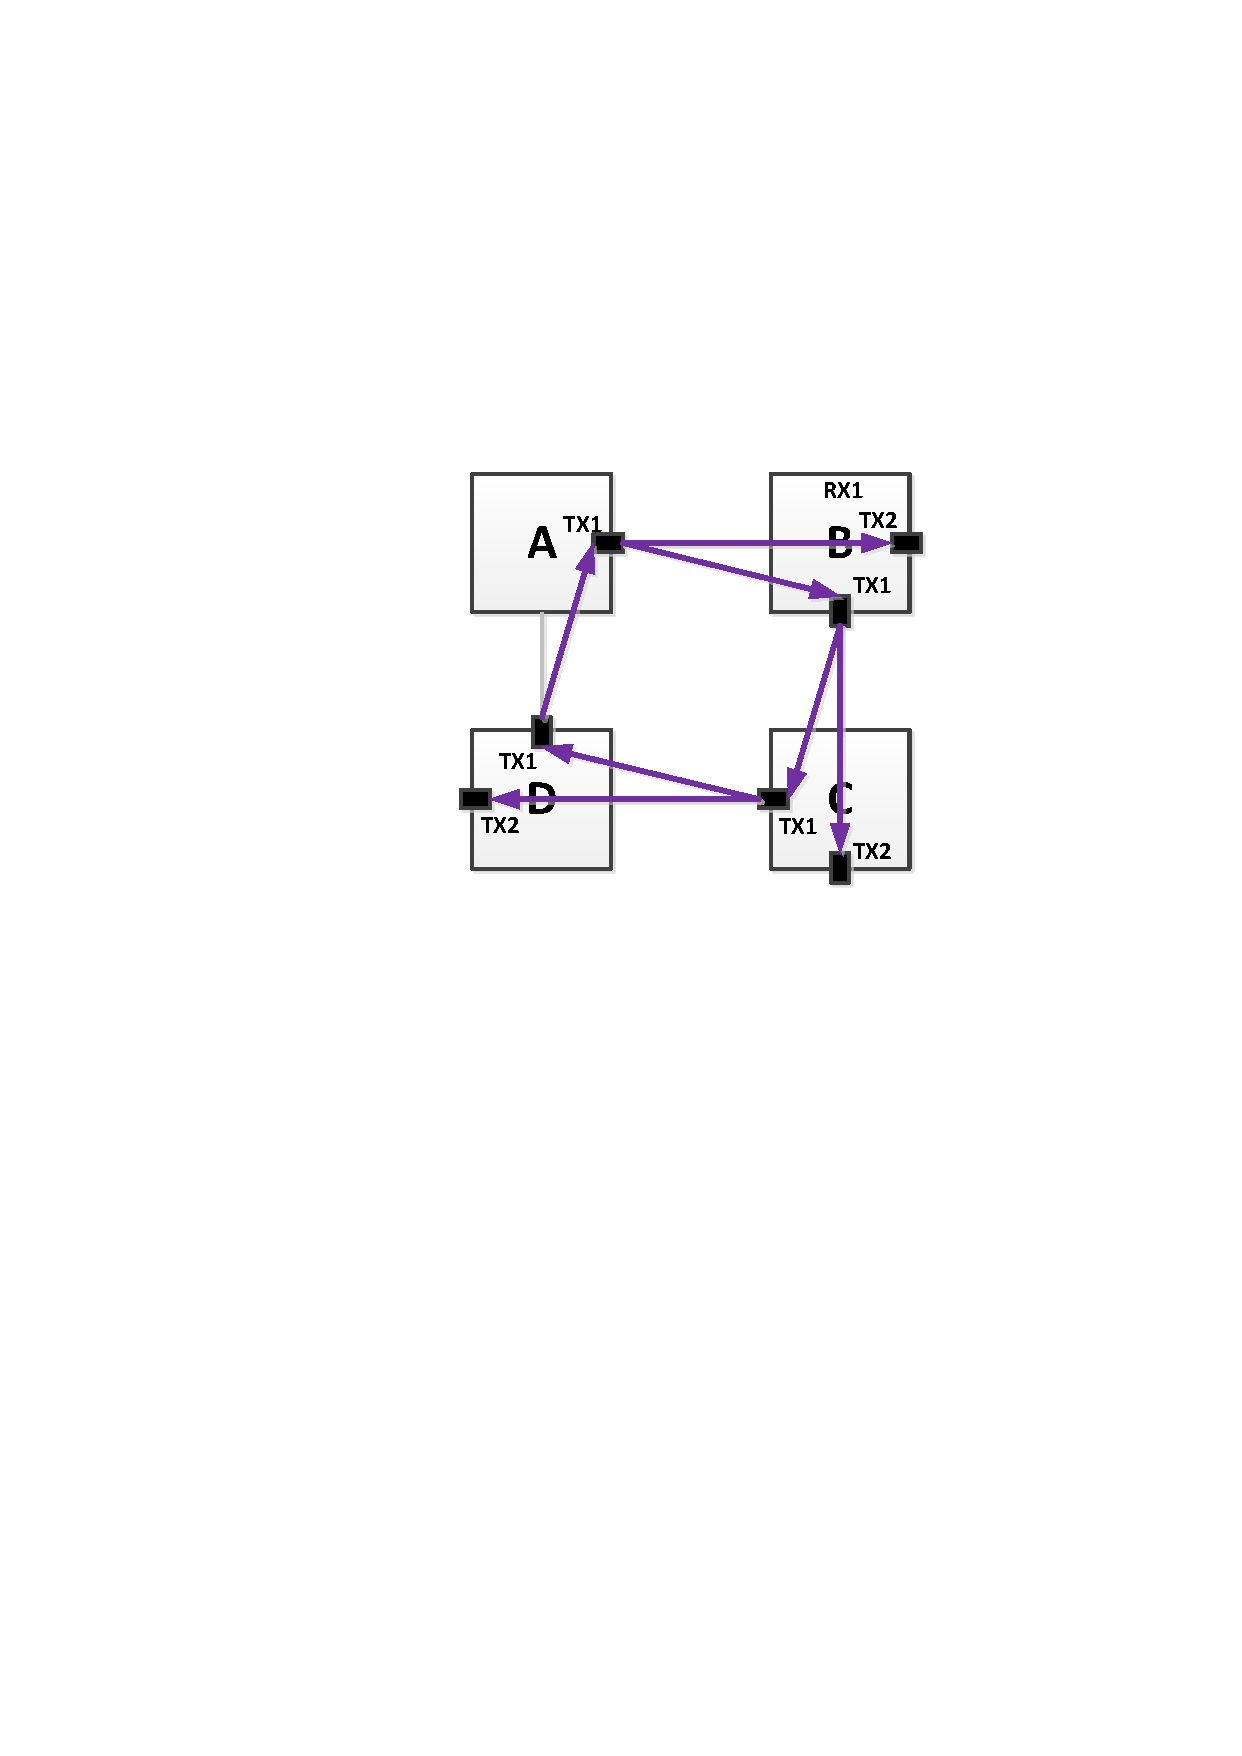
\includegraphics[width=0.27\textwidth] {figs/case2_buffer_dependency}
}
\subfloat[short for lof][Pause events at four links.]{
    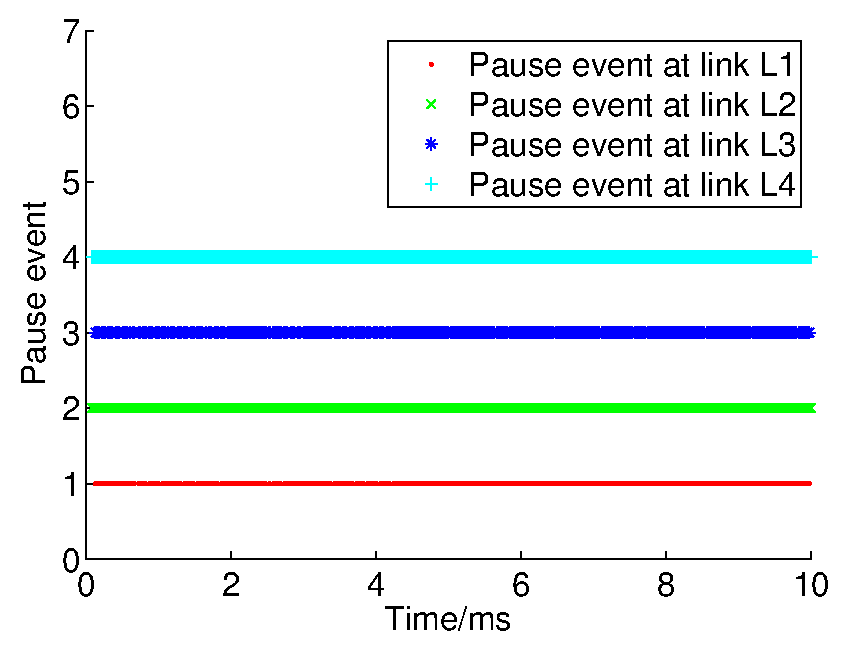
\includegraphics[width=0.3\textwidth] {figs/case2_pause.eps}
}


\caption{Deadlock case 2.}\label{fig:case2}

\end{figure*}

\textbf{Case 1:} In this case, as shown in Fig.~\ref{fig:case1}(a), we let two flows run over four switches A, B, C and D. Flow 1 starts at a host (not shown) attached to A, passes through B and C, and ends at a host attached to D. Flow 2 starts at a host attached to C, passes through D and A, and ends at a host attached to B. In the figure, RX represents input queue (or port), while TX represents output queue (or port). To evaluate whether there will be deadlock in the worst case, both flows are UDP flows with infinite traffic demand.

Buffer dependency graph of case 1 is drawn in Fig.~\ref{fig:case1}(b). Each directed line represents a buffer dependency from the source TX to the destination TX. For example, packets buffered in TX1 of A will be sent to either TX1 or TX2 of B, so in Fig.~\ref{fig:case1}(b), two directed lines are drawn there between A and B. Similarly, we can draw the dependency lines between other switches. As we can see in Fig.~\ref{fig:case1}(b), there is a cyclic buffer dependency among the four switches, i.e., dependencies from TX1 of A to TX1 of B, then to TX1 of C, then to TX1 of D, and finally back to TX1 of A.

In Fig.~\ref{fig:case1}(c), we plot the PFC pause events at four links L1, L2, L3 and L4. Basically, if link Li (i=1,2,3,4) is paused at time t, we plot a point at location (t, i). Pause events at different links are plotted with different colors and of different heights. As we can observe, links L2 and L4 are paused continuously, while the other two links L1 and L3 never get paused. In this case, deadlock will never occur as no packet will be paused permanently.

To understand the pause pattern in Fig.~\ref{fig:case1}(c), we sample the instant buffer occupancy of both flows at TX1 queues of A, B, C and D every 1us. In Fig.~\ref{fig:case1}(d), we draw the instant buffer occupancy of flow 2 at TX1 of A. Buffer occupancy of flow 1 is not drawn in Fig.~\ref{fig:case1}(d) as it does not contribute to the pause of link L1 (Note that PFC works in a per ingress queue fashion). 

Similarly, in Fig.~\ref{fig:case1}(e), Fig.~\ref{fig:case1}(f) and Fig.~\ref{fig:case1}(g), we draw the instant buffer occupancy of interested flows at TX1 queues of B, C and D, respectively. As flow 1 and flow 2 are symmetric, we only present the analysis for Fig.~\ref{fig:case1}(d) and Fig.~\ref{fig:case1}(e) to show why Link L4 is paused continuously but link L1 never gets paused.

As shown in Fig.~\ref{fig:case1}(d), buffer occupancy of flow 2 at TX1 of A fluctuates between 10KB and 55KB around the PFC threshold, so link L4 will get paused intermittently. In contrast, buffer occupancy of flow 1 at TX1 of B is well below the PFC threshold (fluctuates between 0KB and 18KB), hence link L1 will never be paused.

%In Fig.~\ref{fig:case1}(a), packets of flow 1 and flow 2 will build up at TX1 of A as both flows are competing for the capacity of link L1. Once the buffer occupancy of flow 2 exceeds the PFC threshold, RX1 of A will generate a pause frame to TX1 of D to stop packet transmission over link L4.
%
%After link L4 is paused, buffer occupancy of flow 2 will decrease as no more packets can be received by RX1 of A. Once the buffer occupancy of flow 2 is below the PFC threshold at switch A, link L4 will be resumed. Then buffer occupancy of flow 2 will start to increase again. This is why in
%
%Since packets of flow 1 buffered in TX1 of B can get transmitted at full link speed when link L2 is not paused, TX1 queue of B can not easily build up. As we can see in Fig.~\ref{fig:case1}(e), buffer occupancy of flow 1 at TX1 of B fluctuates between 0KB and 18KB, which . Hence as we can see in Fig.~\ref{fig:case1}(c), link L1 is never paused by RX1 of C.


\textbf{Observation 1:} Deadlock may not occur when cyclic buffer dependency exists in the network. Cyclic buffer dependency is just a necessary condition for deadlock.



\textbf{Case 2:} as shown in Fig.~\ref{fig:case2}(a), in the second case, in addition to case 1, we add another flow (flow 3) to run over switches B and C in sequence. All the three flows are UDP flows with infinite traffic demand. Buffer dependency graph of case 2 is drawn in Fig.~\ref{fig:case2}(b). Compared with case 1, one additional dependency from TX1 of B to TX1 of C is added.

Pause events at four links L1, L2, L3 and L4 are plotted In Fig.~\ref{fig:case2}(c). As we can see, in this case four links are all paused. To check whether deadlock will occur in this case, we stop the three flows after a sufficient long period (1000ms). What we find is that, pause events are continuously generated at all the four links even after three flows stop sending new packets (not shown in the figure). This means that a deadlock has been created among switches A, B, C and D.

In the next, we will explain why deadlock can be created by adding one additional flow to the network. After adding flow 3, packets of flow 1 buffered in TX1 of B can no longer get transmitted at full link speed due to the contention with packets of flow 3. Packets of flow 1 will then build up at TX1 of B. Once the packets of flow 1 buffered at TX1 of B exceed the PFC threshold, RX1 of B will send a pause frame to TX1 of A to pause Link L1. The pause on link L1 will help packets to build up at TX1 of A, and has a cascade effect on link L4. Due to the pause at link L1, link L4 will get paused more frequently. Then packets of flow 2 are easier to build up at TX1 of D. Once the PFC threshold is triggered at D, link L3 also get paused. So in case 2, pause events can occur at all the four links.

Once all the four links are paused simultaneously, there is a chance that no link can get resumed. For example, it is possible that when simultaneous pause happens, at switch A and switch B, the first packet buffered in the head of TX1 is a packet of flow 1, and meanwhile, at switch C and switch D, the first packet buffered in the head of TX1 is a packet of flow 2. If the above condition occurs, no link can get resumed as all the TX1 queues are waiting for its downstream neighbors to release some buffer to break the standstill condition.

\textbf{Observation 2:} Deadlock will occur when all the links in a cycle are paused simultaneously and no link can get resumed.


\begin{figure*}[t]
%\vspace{-0.1in}
\centering

\subfloat[short for lof][Topology and flows.] {
    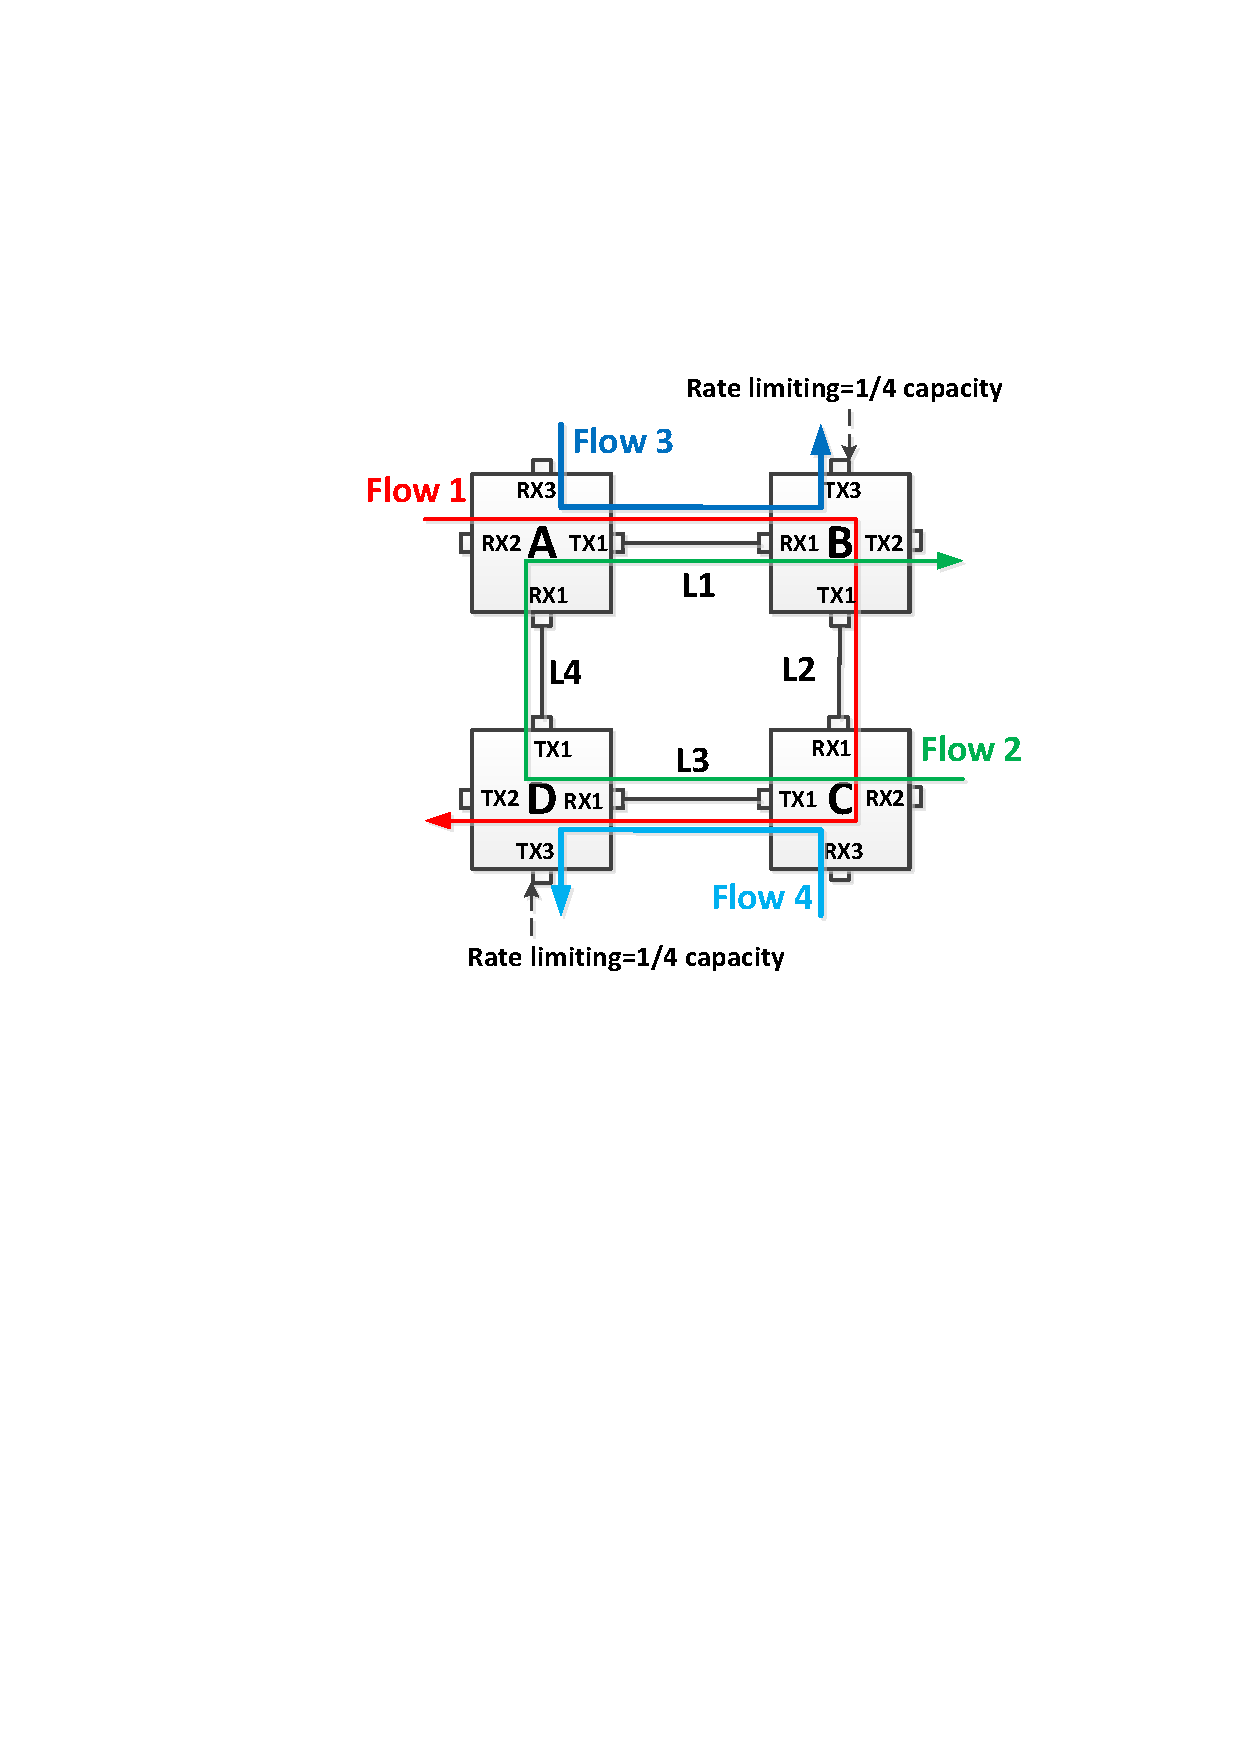
\includegraphics[width=0.37\textwidth] {figs/case3_topo}
}
\subfloat[short for lof][Buffer dependency.]{
    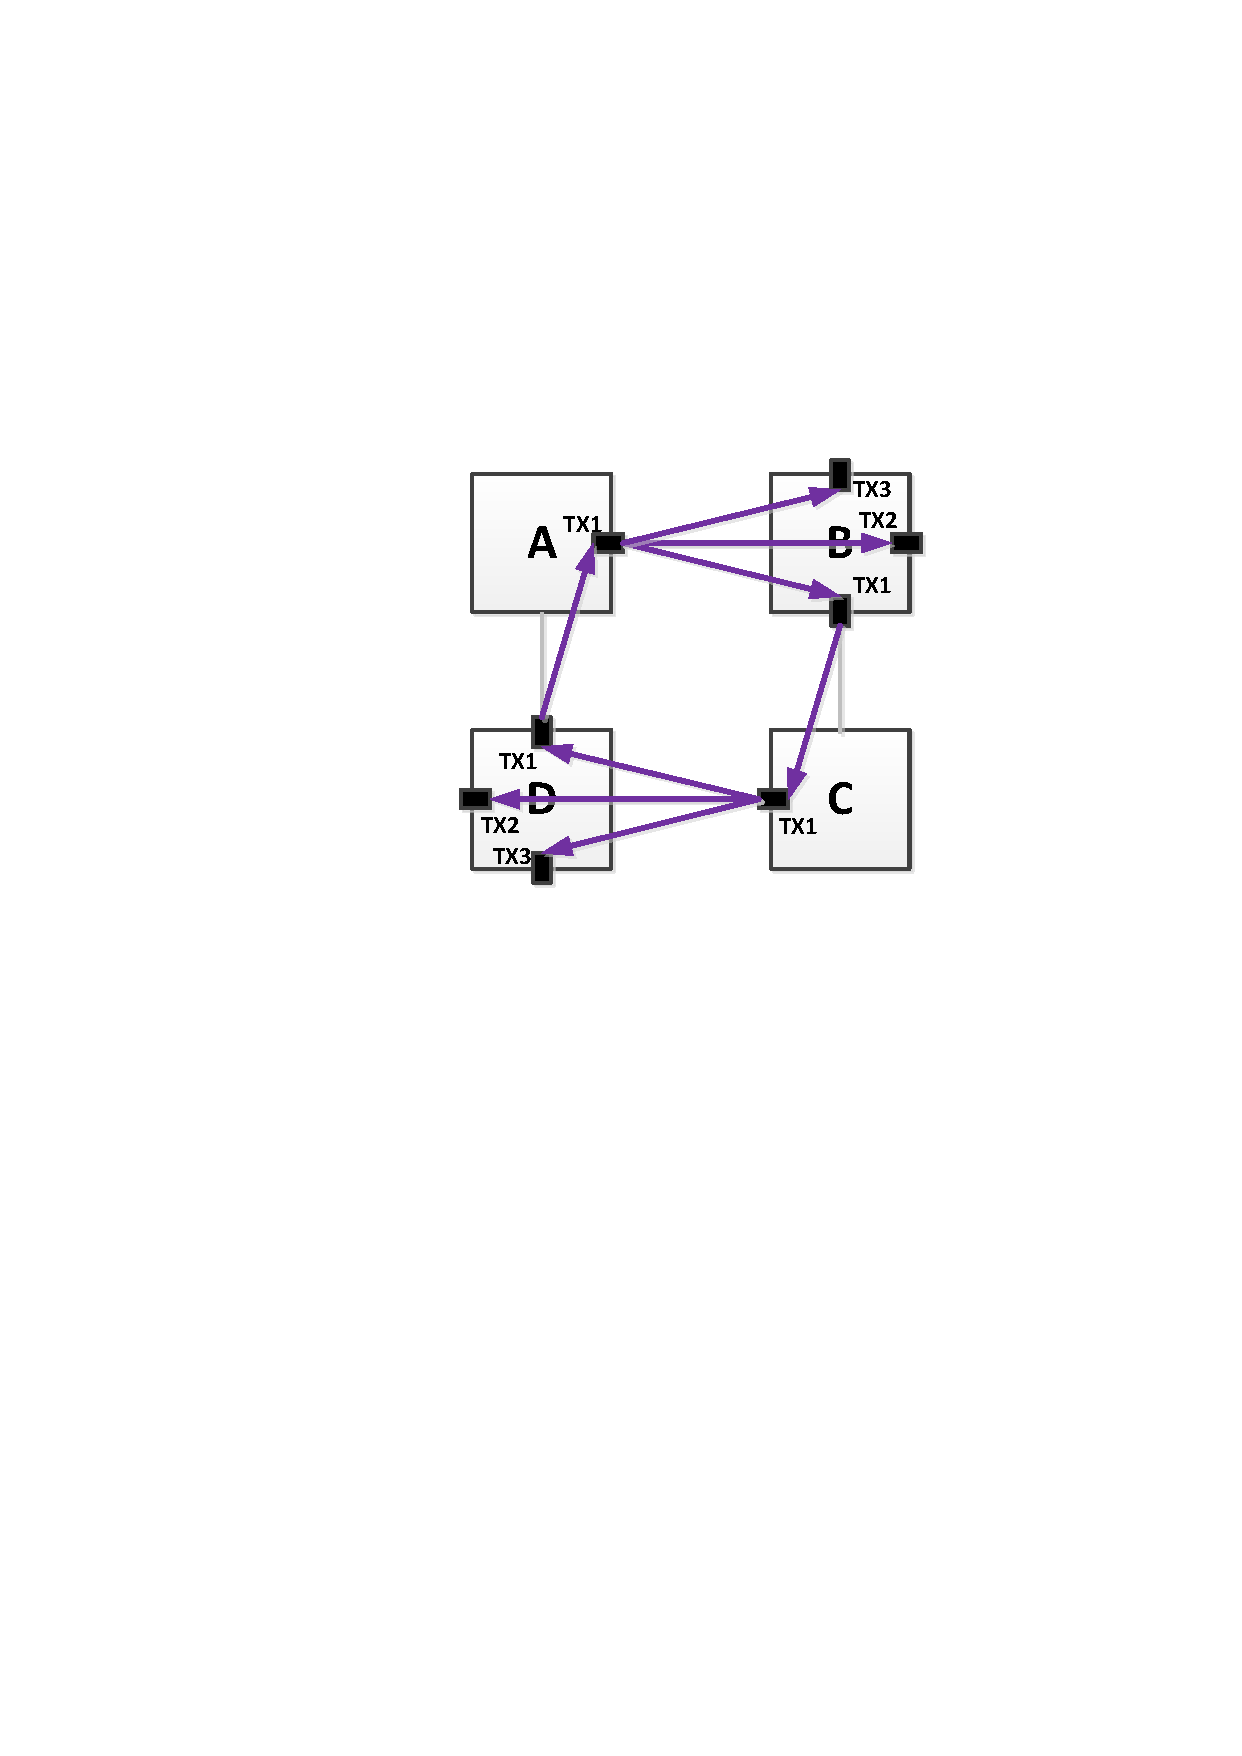
\includegraphics[width=0.28\textwidth] {figs/case3_buffer_dependency}
}
\subfloat[short for lof][Pause events at four links.]{
    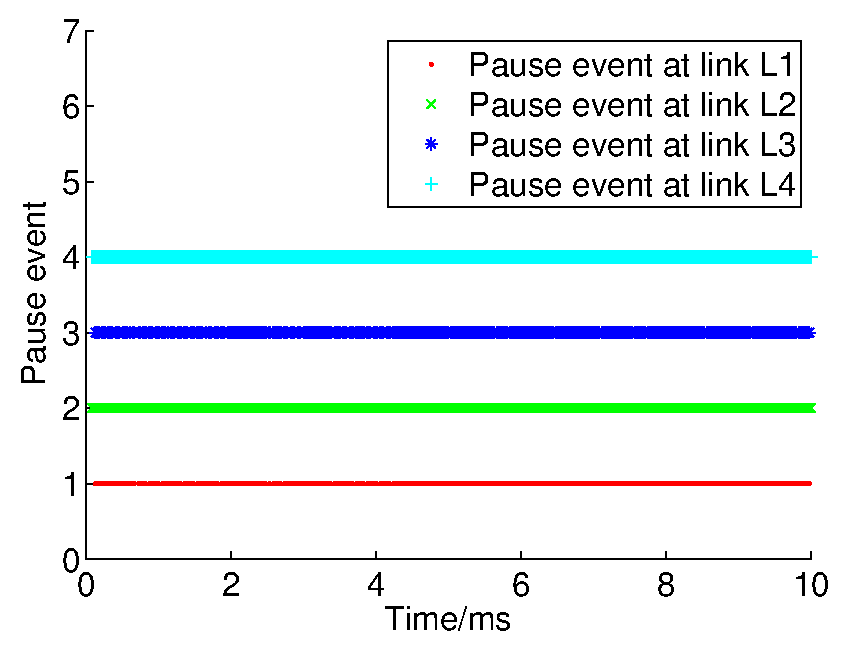
\includegraphics[width=0.3\textwidth] {figs/case3_pause.eps}
}

\subfloat[short for lof][Buffer occupancy of flow 2 at switch A.] {
    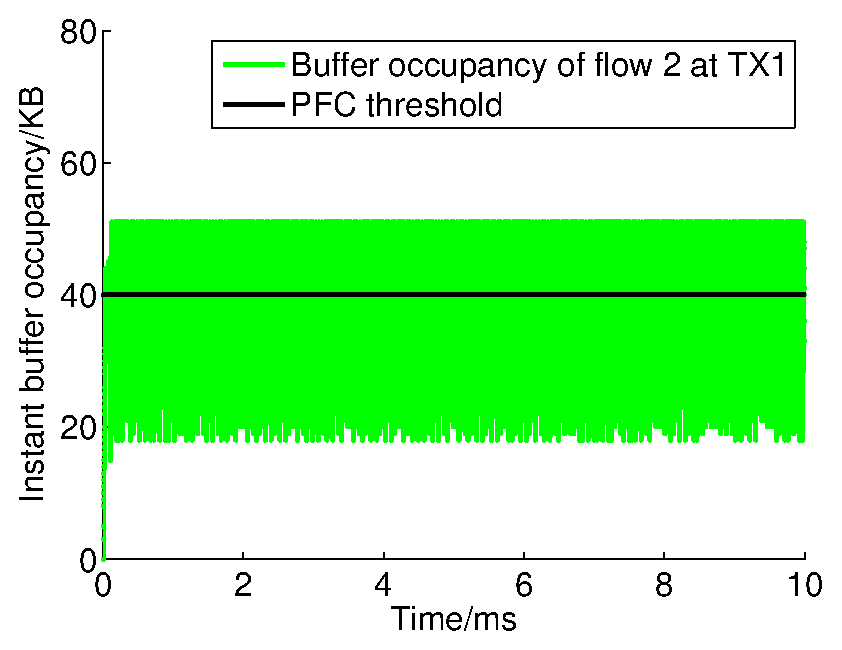
\includegraphics[width=0.33\textwidth] {figs/case3_buffer_occupancy_A.eps}
}
\subfloat[short for lof][Buffer occupancy of flow 1 at switch B.] {
    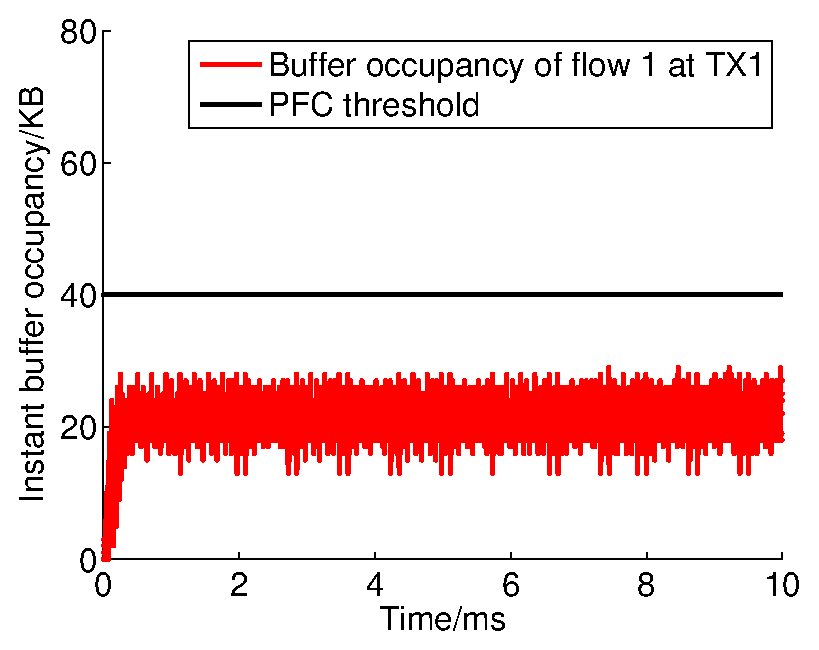
\includegraphics[width=0.33\textwidth] {figs/case3_buffer_occupancy_B1.eps}
}
\subfloat[short for lof][Buffer occupancy of flow 3 at switch B.] {
    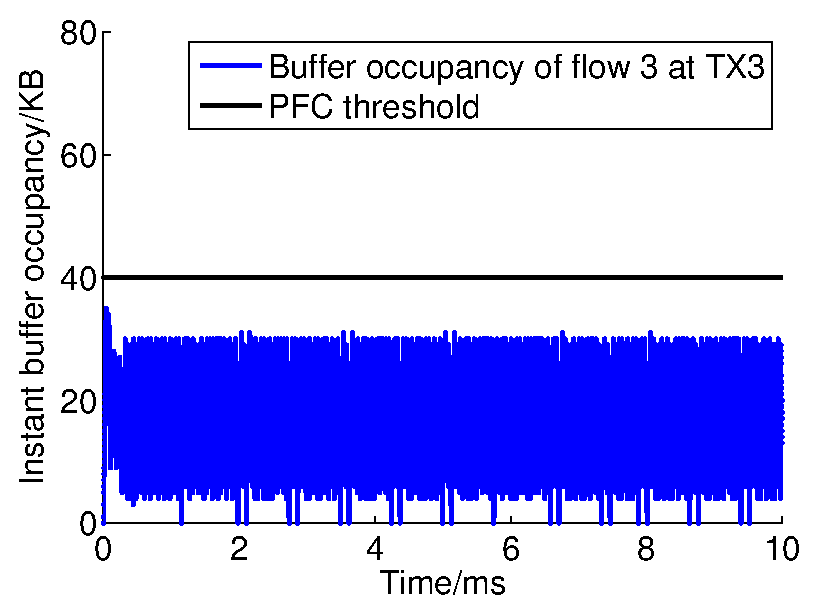
\includegraphics[width=0.33\textwidth] {figs/case3_buffer_occupancy_B3.eps}
}

\caption{Deadlock case 3.}\label{fig:case3}

\end{figure*}

\textbf{Case 3:} In this case, we will show that even if all the four links are paused simultaneously, it is not guaranteed that a deadlock will be created. As shown in Fig.~\ref{fig:case3}(a), in addition to case 1, we add another two flows (flow 3 and flow 4). Flow 3 starts at a host attached to A, passes through A and B, and ends at a host attached to B. Flow 4 is a symmetric flow of flow 3 that runs over C and D. All the four flows are UDP flows with infinite traffic demand. Two rate limiters are added at TX3 queues of B and D to ensure that rates of flow 3 and flow 4 will not exceed $1/4$ of the link capacity. Buffer dependency graph of case 3 is drawn in Fig.~\ref{fig:case3}(b). Compared with case 1, two additional buffer dependencies from TX1 queues to TX3 queues are added.

Pause events at four links L1, L2, L3 and L4 are plotted In Fig.~\ref{fig:case3}(c).  As we can see from the figure, all the four links are paused continuously. However, we find that once we stop the flows, all the links get resumed and buffer occupancy of four switches soon becomes zero. This indicates that deadlock cannot be created in case 3.

To find out why there is no deadlock in case 3, we draw the instant buffer occupancy of 3 flows at switches A and B in Fig.~\ref{fig:case3}(d), Fig.~\ref{fig:case3}(e) and Fig.~\ref{fig:case3}(f). Here we omit the buffer occupancy condition of switches C and D as the topology and the flows are symmetric.

As shown in Fig.~\ref{fig:case3}(d), at TX1 of A, the buffer occupancy of flow 2 exceeds the PFC threshold, so link L4 will get paused. To understand why link L1 is also paused, we need to consider the buffer occupancy of flow 1 and flow 3 at switch B. The reason is that packets received by RX1 of B are possible to be queued at both TX1 and TX3 (note that there is a rate limiter on TX3). As long as the sum of the buffer occupancies of both TX queues exceeds the PFC threshold, link L1 will get paused. As we can see in Fig.~\ref{fig:case3}(e) and Fig.~\ref{fig:case3}(f), although individually buffer occupancy of either TX1 or TX3 is less than the PFC threshold, their sum is larger than the PFC threshold. Hence link L1 is paused.

As both TX1 and TX3 contribute to the pause on link L1, to create a deadlock, we need to ensure that packets buffered at both TX queues cannot get resumed. However, packets buffered at TX3 can always get transmitted within a finite time as it is not involved in any cyclic buffer dependency. This explains why when we stop the flows, all the four links can be resumed from the pauses. 


\textbf{Observation 3:} even if all the links in a cycle are paused simultaneously, it is not sufficient to create a permanent deadlock.

%\subsection{Deadlock problem in RDMA DCNs}\label{subsec:deadlock_problem}
%
%Once a loop occurs in a network, packets of some flows will be caught in the loop and traverse the same links multiple times until they are dropped due to Time-to-Live (TTL) expiration. Apart from causing packet drops, loops will also waste some link bandwidth as well as increase the end-to-end delay for the flows traversing some link(s) in the loop (but not caught by the loop).
%
%\begin{figure}[t]
%\centering
%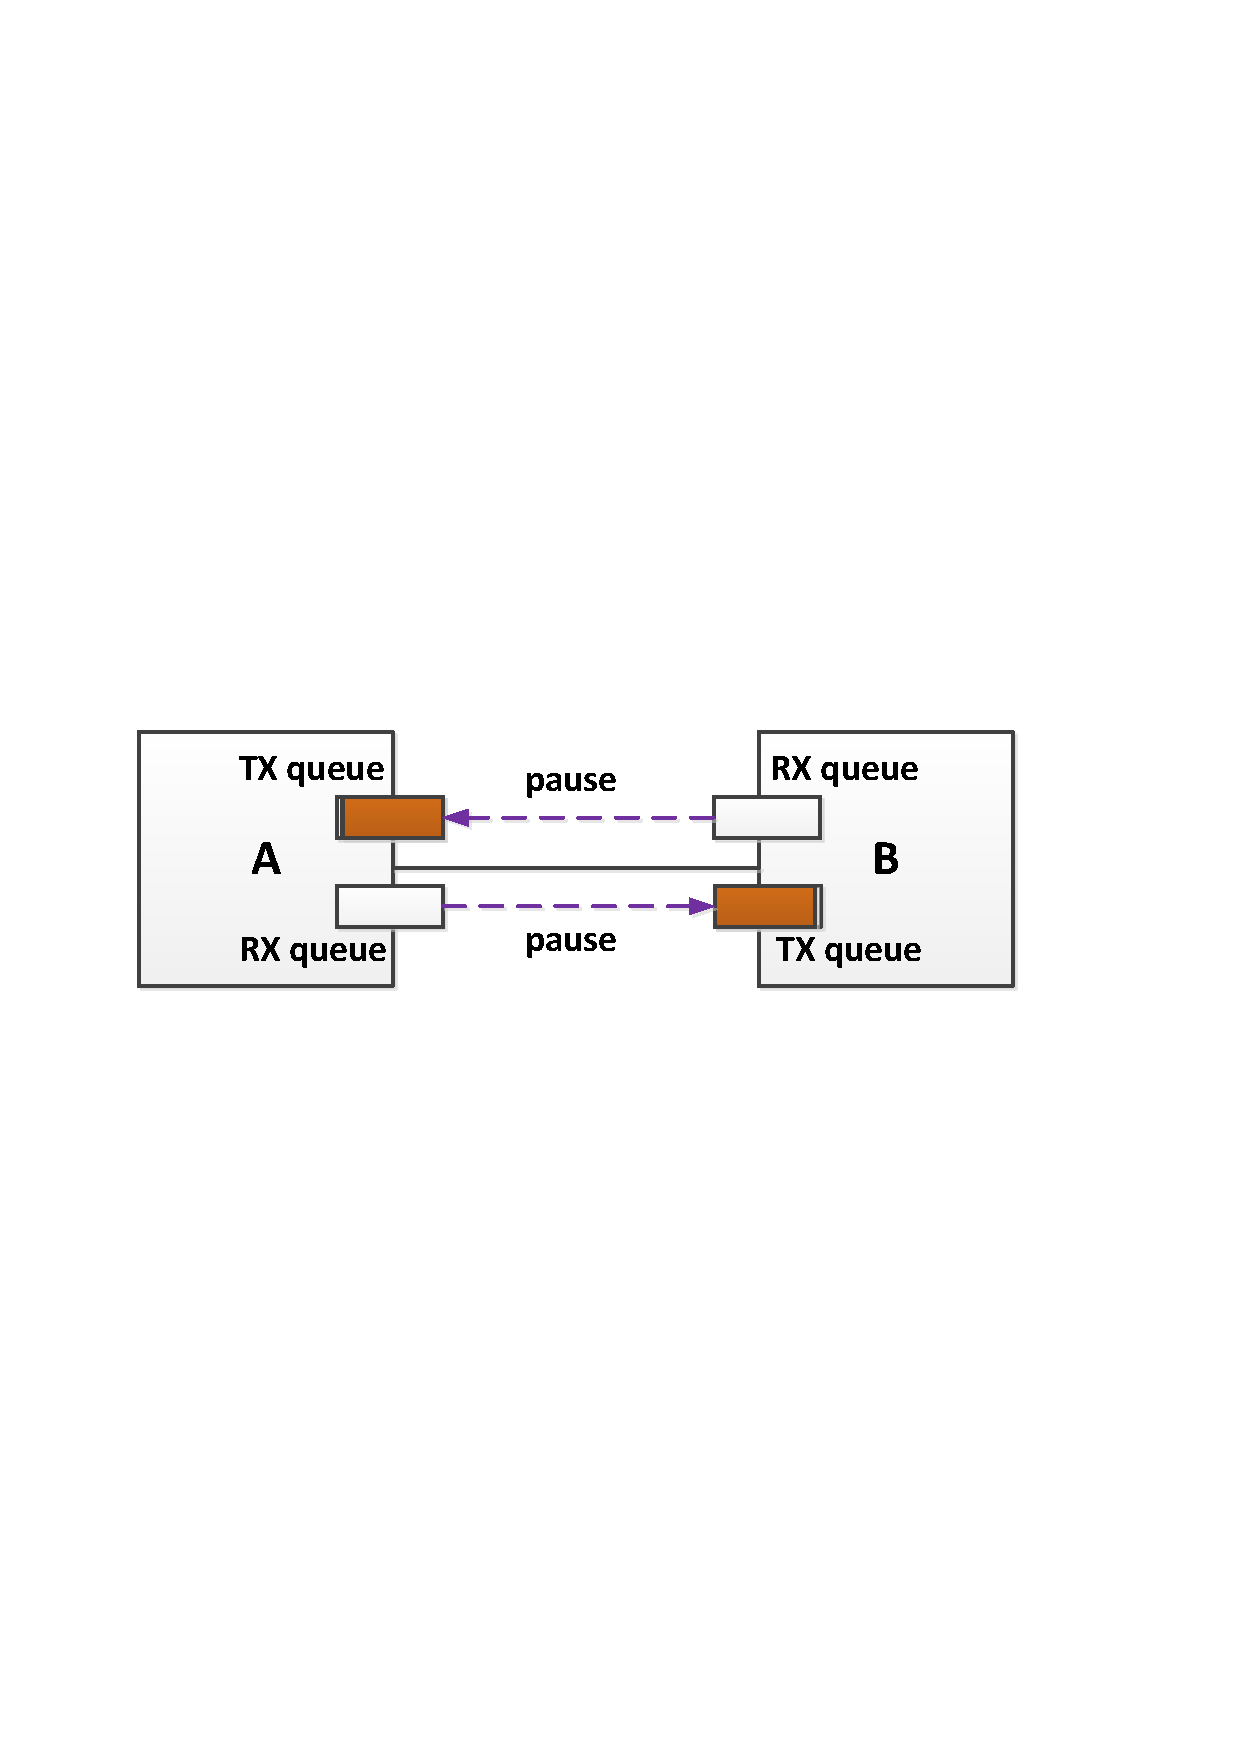
\includegraphics[width=0.45\textwidth,center]{figs/deadlock_example.pdf}
%\caption[Optional caption for list of figures]{An example of loop induced deadlock: there is a loop between switch A and switch B. Both TX queues (egress queues) are paused by PFC as no buffer are available at both switches to accommodate more packets.}
%\label{fig:loop_deadlock}
%\end{figure}
%
%In a lossy network, the impact of a loop is not fatal and can be completely eliminated as long as the loop is removed from the network. In contrast, in a lossless network, if packets enter a loop faster than they get dropped in the loop due to TTL expiration, packets will occupy the buffer of all the switches in the loop, and then a deadlock is created. When a deadlock occurs, each switch in the loop is paused by its downstream switch, and at the same time pauses its upstream switch due to the lack of available buffer to accept more packets. Once such a circular buffer dependency is created, the deadlock condition will hold persistently even after the loop is eliminated.
%
% Under deadlock condition, no packets can move along the links in the loop, and more and more devices outside the loop will be paused due to the cascade effect of PFC. If a deadlock is created in the core of the network, it is very likely to bring the whole data center into a deadlock state.
%
%A simple deadlock example is shown in Fig.~\ref{fig:loop_deadlock}. In this example, there is a routing loop between switch A and switch B. Packets enter this loop at a sufficient large rate and soon occupy all the available buffer of both switches. Then Both TX queues (egress queues) will be paused by PFC PAUSE frames and a deadlock is created. As we can see, this deadlock cannot be resolved by eliminating the routing loop as packets are already queued in the TX queues and can never reach the next-hop switch to escape from the loop.
%
%\subsection{Sufficient condition for deadlock creation}\label{subsec:deadlock_condition}
%
%In this part, we analyze the sufficient condition to create a deadlock when there is a loop in the network.
%
%At first, we consider the maximum packet drain rate in a loop regarding TTL expiration. Let $n$ the number of switches in a loop, $B$ be the link bandwidth and $k_{TTL}$ be the TTL value of packets before they enter the loop. Each time a packet traverses one switch, its TTL value will be reduced by 1.
%
%The maximum packet drain rate is achieved when no switch is paused by PFC PAUSE frame and each switch is sending packets to its next-hop in the loop at the rate of $B$. So the maximum packet drain rate $r^{max}_d$ is equal to $nB/k_{TTL}$. here $nB$ can be viewed as the maximum packet ``flowing" rate in the loop, while $1/k_{TTL}$ captures the information that a packet will be dropped after it has traversed $k_{TTL}$ hops of switches in the loop.
%
%Let $r_{in}$ be the injection rate of packets into the loop. One sufficient condition to create a deadlock in a lossless network is that: there is a loop
%in the network, and condition $r_{in} > r^{max}_d$ holds for a sufficient long period until a circular buffer dependency is created in the loop.
%
%\begin{figure}[t]
%\centering
%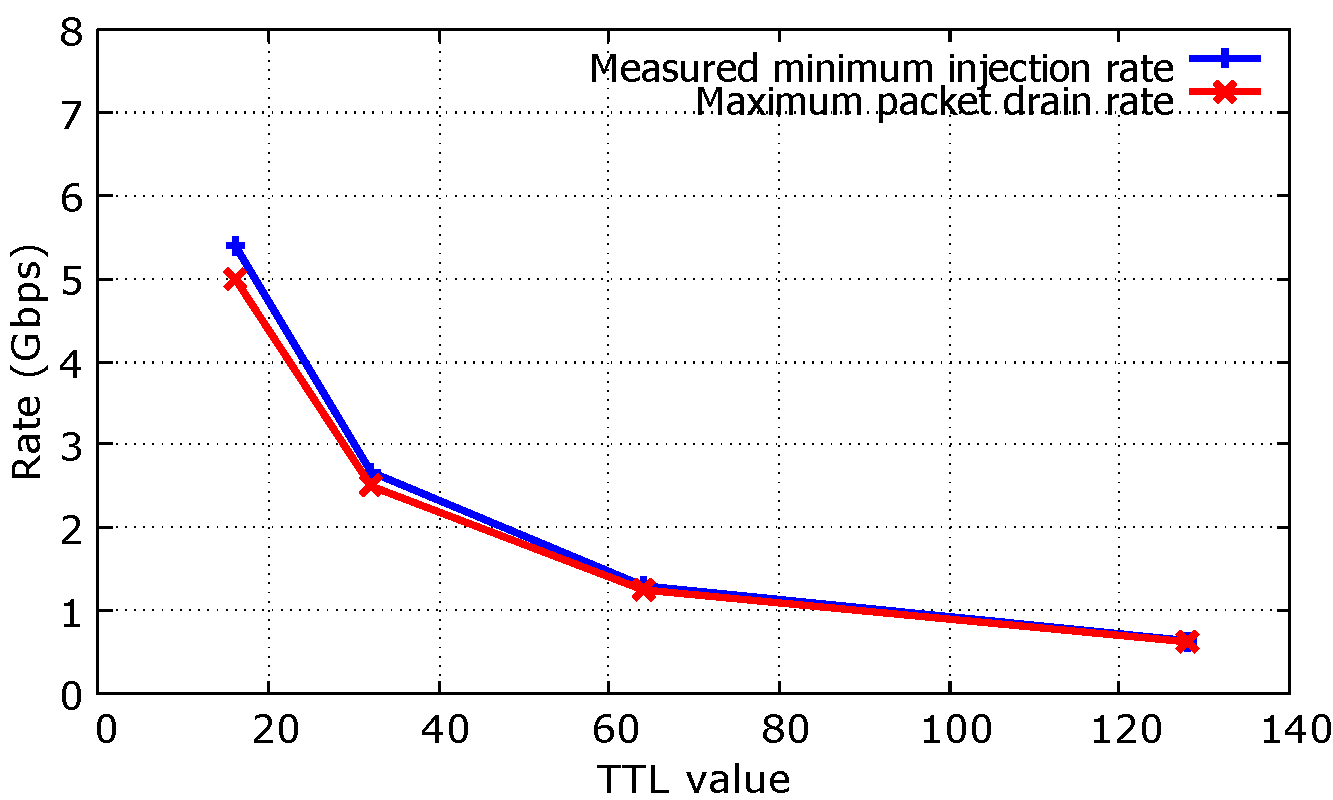
\includegraphics[width=0.5\textwidth,center]{figs/r_and_rdrain.pdf}
%\caption[Optional caption for list of figures]{Measurement of the minimum injection rate to create a deadlock. Both switches in the loop are Arista 7050QX32.}
%\label{fig:mrate_measurement}
%\end{figure}
%
%To verify our analysis above, we manually configure a loop between two 40Gbps switches, and measure the minimum packet injection rate that can create a deadlock. The result is shown in Fig.~\ref{fig:mrate_measurement}. As we can see, the measured minimum packet injection rate is just slightly larger than the maximum packet drain rate which is computed according to $nB/k_{TTL}$. This observation holds when TTL is set to different values.
%
%Another observation from the figure is that, setting smaller TTL can help to prevent deadlock but its benefit is limited. As shown in the figure, when TTL is set to 16 which is already a very small value, the minimum injection rate is only about 6Gbps.
%
%\subsection{Analysis of the time to create a deadlock}\label{subsec:deadlock_condition}
%
%In this part, we analyze and measure the time to create a deadlock when the sufficient condition for deadlock creation is already met. Deadlock creation time is related to three factors: \textbf{packet injection rate $r_{in}$}, \textbf{packet drain rate $r_{d}$} and \textbf{PFC threshold $t_{PFC}$}.
%
%$t_{PFC}$ determines the minimum bytes of packets needed to be ``trapped" in the loop to create a deadlock, while $r_{in} - r_{d}$ can be viewed as the packet increase rate.
%
%%Packet injection rate is determined by the instant traffic demand of applications running in the data center. A larger injection rate requires less time to create a deadlock.
%%
%%As discussed above, the maximum packet drain rate will be a fixed value once $n$, $B$ and $k_{TTL}$ is determined. We find that packet drain rate will decrease significantly after packets are queued in the loop because it will take a packet much longer time to get dropped in the loop when there is queuing delay.
%
%Most modern commodity switches use a dynamic $\alpha$ algorithm to determine the value of PFC threshold: Let $\alpha$ be a parameter with the range from 0 to 1, $m$ be the total switch buffer size and $m^\prime$ be the amount of buffer currently occupied. For a given $\alpha$, the value of $t_{PFC}$ is dynamically computed according to the following equation $ t_{PFC} = \alpha(m - m^\prime)$. During runtime, once the queue length of an ingress queue exceeds the instant $t_{PFC}$, a PAUSE frame will be sent to its upstream device. Note that a PAUSE frame will take some time to arrive an upstream device and take effect. To avoid packet loss due to this delay, some buffer headroom must be reserved for each ingress queue, and hence the value of $m$ in the equation is usually slightly smaller than the total switch buffer size.
%
%%
%
%
% %Most modern commodity switches share memory buffer among all ports. In order to better utilize the available shared buffer in a timely fashion, instead of setting a fixed PFC threshold,
%%A PAUSE frame will take some time to arrive an upstream device and take effect. To avoid packet loss due to this propagation delay, we must reserve enough
%%buffer headroom for each ingress queue to accommodate packets a switch may receive before a PAUSE frame finally takes effect. Let $\Delta m$ be the total amount of reserved buffer headroom. The $m$ in the above equation should be modified to be $m - \Delta m$.
%%Switches and NICs will track the value of $m^\prime$ and update the value of $t_{PFC}$ during runtime.
%
%%A smaller $\alpha$ value can lead to a shorter creation time of deadlock.  This is because a smaller $\alpha$ value means a smaller PFC threshold, while a smaller PFC threshold requires less packets to trigger a switch queue to send PAUSE frames to stop its upstream neighbors.
%
%In the next, we measure the time to create a deadlock when setting different $\alpha$ and TTL values.
%
%
%\begin{figure}[t]
%\centering
%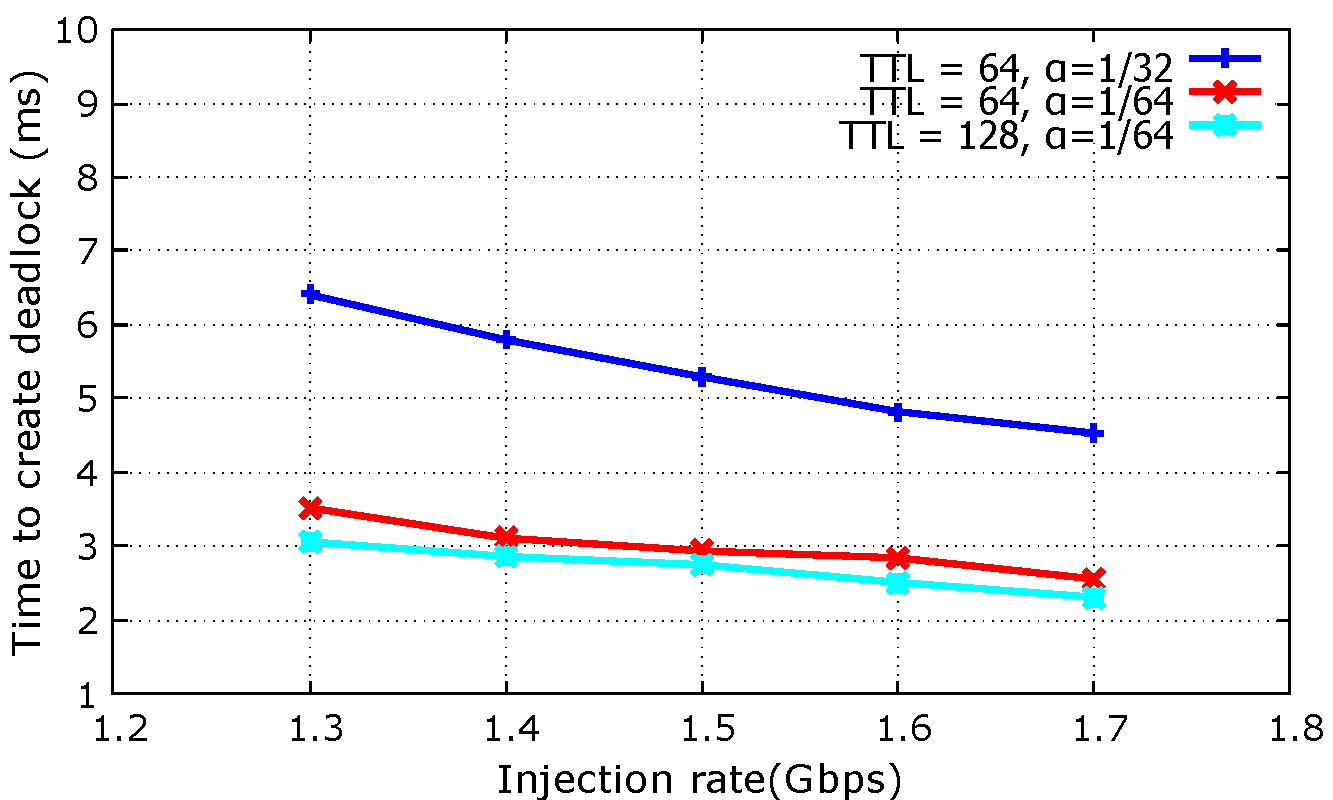
\includegraphics[width=0.5\textwidth,center]{figs/r_dltime.pdf}
%\caption[Optional caption for list of figures]{Measurement of the time to create a deadlock under different settings (deadlock will not occur when the injection rate is less than 1.3Gbps).}
%\label{fig:dltime_measurement}
%\end{figure}
%
%\parab{Measurement of the time to create a deadlock:} We manually configure a loop between two Arista 7050QX32 switches which have 32 full duplex 40Gbps ports and 12MB shared buffer. In Fig.~\ref{fig:dltime_measurement}, we set $\alpha$ and $TTL$ to different values and measure the time to create a deadlock under different injection rates.
%
%We can make four observations from the results in Fig.~\ref{fig:dltime_measurement}: 1) It takes only a few milliseconds to create a deadlock even when the injection rate is less than 2Gbps. This indicates that it is easy for a deadlock to occur even when only a transilient loop exists in the network. In addition, we cannot rely on any loop detection and recovery solutions to prevent the occurance of deadlocks as they are too slow to resolve the loop within a few milliseconds. 2) As the injection rate increases, the time to create a deadlock decreases accordingly. 3) Given a fixed injection rate, a smaller $\alpha$ value requires less time to create a deadlock. 4) Given a fixed injection rate, a smaller TTL value requires more time to create a deadlock. This is because a smaller TTL value will make the packets get dropped faster in the loop, and thus more packets are needed to be injected into the loop to trigger switch to pause each other.
%
%We repeated this experiment using many other combinations of TTL and $\alpha$ values and different number of switches. We found that all the results comply with what have been shown in Fig.~\ref{fig:dltime_measurement}.
%
%The takeaway of this experiment is that: once there is a loop in the network, deadlock is easy to occur and very hard to prevent (a deadlock can be created within a few milliseconds). In addition to a fast loop detection mechanism, we need an effective solution to detect and resolve deadlocks caused by all kinds of loops.

%\parab{Estimation of the time to create a deadlock:}

%\parab{Sufficient condition for deadlock creation:} \todo{(detailed content to be added later.)}
%
%   1. Analysis of the maximum packet drain rate caused by TTL expiration: $r^{max}_d = nB/k_ttl$.
%
%   2. Using testbed experiments to demonstrate that $r > r^{max}_d$ is a sufficient condition for deadlock creation.
%
%\parab{Creation time of deadlock:} \todo{(detailed content to be added later.)}
%
%   1. Analysis of the upper bound and lower-bound of the creation time of deadlock.
%
%   2. a) Using testbed experiments to demonstrate that lower-bound value is already a tight estimation when $r << B$; b) Analysis of the impact of PFC PAUSE frames on $r$ and $r^{max}_d$.
%
%\subsection{Analysis of device bug induced deadlock}\label{subsec:analysis_loop_deadlock}
%\todo{to be added.}
